\documentclass[fleqn,10pt]{physiome}
% Use option lineno for line numbers 

\articletype{Original}
%% Choose from Original, Retrospective, Review, Letter
\usepackage{supertabular}

\title{Computational Modeling of Coupled Energetics and Mechanics in the Rat Ventricular Myocardium}

\author[1]{Bahador Marzban}
\author[1]{Rachel Lopez}
\author[1][beardda@umich.edu]{Daniel A. Beard}
\affil[1]{Molecular and Integrative Physiology, University of Michigan, Ann Arbor, Michigan, USA}

%% The following lines can be omitted when submitting;
%% information will be added by editors
\publicationdate{24 Sept. 2020}
\editor{David P. Nickerson}
\curator{Anand K. Rampadarath}
\submitteddate{15 Sept. 2020}
\accepteddate{15 Sept. 2020}
\citethisas{Marzban et al. (2020) Computational Modeling of Coupled Energetics and Mechanics in the Rat Ventricular Myocardium. Physiome.}{10.36903/physiome.12964970}
\begin{document}

\maketitle

\begin{abstract}
This paper details a multi-scale model computational model of myocardial energetics---oxidative ATP synthesis, ATP hydrolysis, and phosphate metabolite kinetics---and myocardial mechanics used to analyze data from a rat model of cardiac decompensation and failure. Combined, these two models simulate cardiac mechano-energetics: the coupling between metabolic production of ATP and hydrolysis of ATP to generate mechanical work. The model is used to predict how differences in energetic metabolic state  found in failing versus control hearts causally contribute to systolic mechanical dysfunction in heart failure. This {\em Physiome} paper describes how to access, run, and manipulate these computer models, how to parameterize the models to match data, and how to compare model predictions to data.
\end{abstract}

\keywords{cardiac energetics, cardiac mechanics, heart failure, mechano-energetic coupling, multi-scale modeling}

\primarypubs[10.36903/physiome.12964970]{sample}{Lopez2020}

\section{Introduction}

The multi-scale modeling approach is summarized in Fig.~\ref{fig:overview}. Model components representing myocardial metabolism \cite{Bazil2016}, myocardial cell mechanics \cite{Tewari2016a,Tewari2016b}, myocardial whole-organ pumping \cite{Lumens2009}, and a simple lumped circulatory model are integrated together to simulate whole-body cardiovascular function. 

All computer codes are available at https://github.com/beards-lab/Rat-Cardiac-Energetic. 
 
\begin{itemize}

\item
The cardiac metabolic energetic model component is parameterized to match data from individual animals based on the oxidative capacity and cytoplasmic metabolite pools obtained from \cite{Lopez2020}. 

\item
Certain parameters from the cross-bridge and calcium-activation models of \cite{Tewari2016a,Tewari2016b} and \cite{Campbell2018} are re-estimated to match data from \cite{Janssen2002} on calcium transients and force-generation in isolated rat cardiac trabeculae, as detailed below.

\item
Wall volumes and anatomic parameters associated with the \cite{Lumens2009} heart model are identified based on anatomical data obtained from echocardiography and ex-vivo gross morphological measurements on individual animals from \cite{Lopez2020}.

\item
The simple lumped parameter circulatory model is identified based on cardiovascular state variables measured under resting conditions. 
\end{itemize}

The resulting integrated model is used to predict the in vivo mechanical function and energetic state of the myocardium under resting conditions in each animal. 

\begin{figure}[ht]\centering
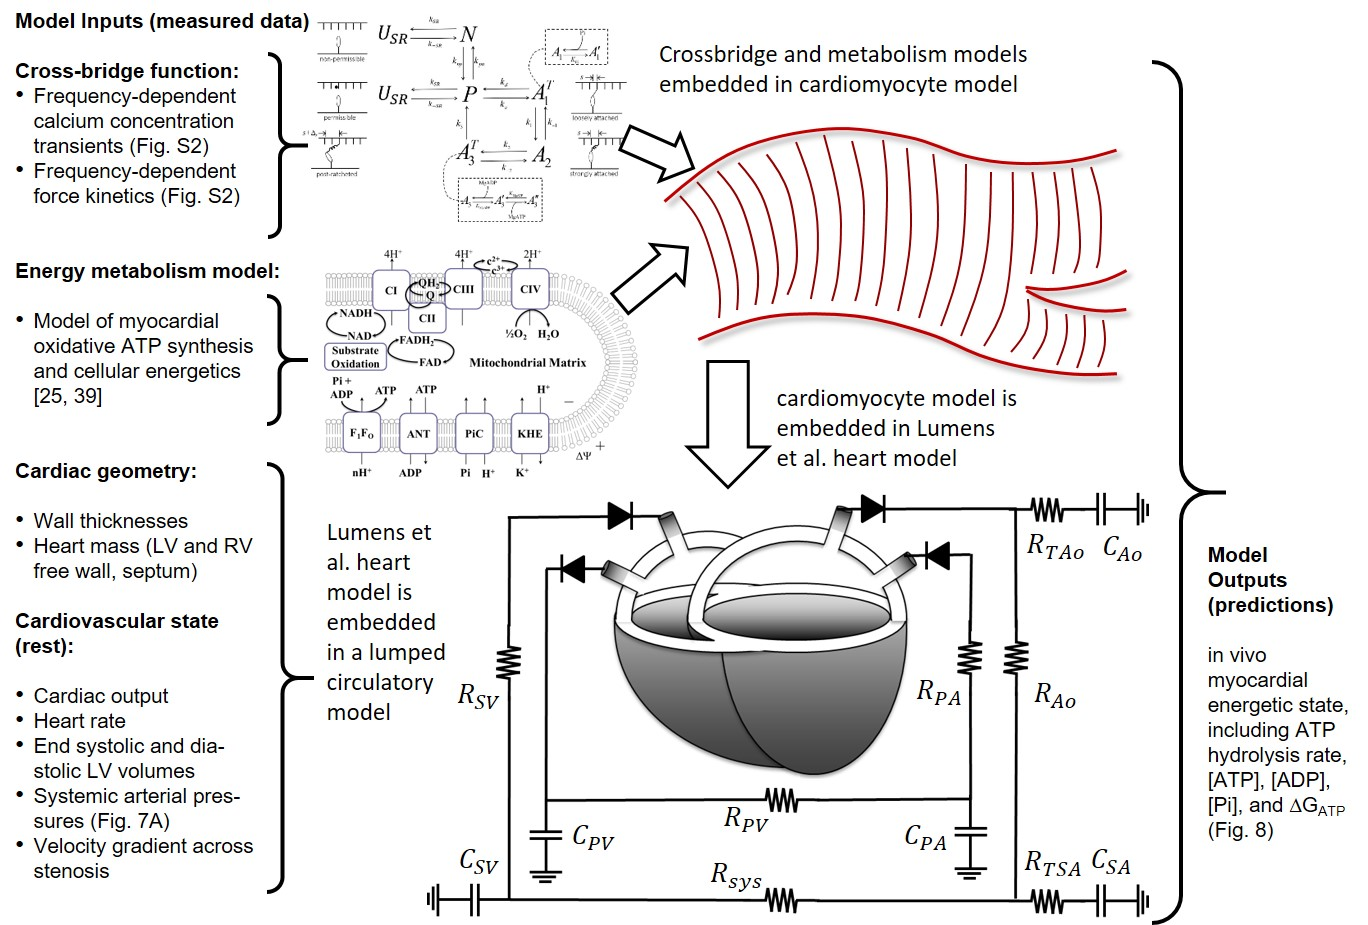
\includegraphics[width=1.0\linewidth]{Figure1}
\caption{Multi-scale modeling of myocardial mechano-energetic function. The model integrates previously developed and validated models of cardiomyocyte dynamics \cite{Tewari2016a,Tewari2016b}, myocardial energetics \cite{Bazil2016, Gao2019}, whole-organ cardiac mechanics \cite{Lumens2009} and a simple lumped parameter closed-loop circulatory system representing the systemic and pulmonary circuits. Data from multiple experimental modalities are used to identify model components for each individual animal in this study. The model predicts variables representing the in vivo myocardial energetic state, including ATP hydrolysis rate, [ATP], [ADP], [Pi], and the free energy of ATP hydrolysis DGATP in the LV myocardium for each individual animal. Figure reproduced from \cite{Lopez2020}.}
\label{fig:overview}
\end{figure}

\section{Model of Cardiac Energy Metabolism}

\subsection{Model Variables:}

\begin{table}[ht]\centering
\caption{Energetics Model State Variables}\label{tab:1}
\begin{tabular}{l l l l}
\toprule
State Variable  & Definition & Units & Variable name in code \\
\midrule
$\Delta\Psi$    & Mitochondrial membrane potential      & mV & DPsi\_im\_to\_matrix \\
\multicolumn{4}{l}{\em Mitochondrial Matrix State Variables} \\
{[ATP]}$_x$       & Total matrix ATP concentration        & M  & ATP\_matrix \\
{[ADP]}$_x$       & Total matrix ADP concentration        & M  & ADP\_matrix \\
{[Pi]}$_x$        & Total matrix Pi concentration         & M  & Pi\_matrix \\
{[NADH]}$_x$      & Total matrix NADH concentration       & M  & NADH\_matrix \\
{[NAD]}$_x$       & Total matrix NAD concentration        & M  & NAD\_matrix \\
{[UQH2]}$_x$      & Total matrix ubiquinol concentration  & M  & coQH2\_matrix \\
{[UQ]}$_x$        & Total matrix ubiquinone concentration & M  & coQ\_matrix \\
{[H$^+$]}$_x$     & Matrix free proton concentration      & M  & h\_matrix \\
{[K$^+$]}$_x$     & Matrix free potassium concentration   & M  & k\_matrix \\
{[Mg$^{2+}$]}$_x$ & Matrix free magnesium concentration   & M  & m\_matrix \\
\multicolumn{4}{l}{\em Intermembrane Space (IMS) State Variables} \\
{[c$^{2+}$]}$_i$  & Total cytochrome c$^{2+}$ (reduced) concentration & M  & cytocred\_im \\
{[c$^{3+}$]}$_i$  & Total cytochrome c$^{3+}$ (oxidized) concentration & M  & cytocox\_im \\
{[ATP]}$_i$       & Total IMS ATP concentration      & M  & ATP\_matrix \\
{[ADP]}$_i$       & Total IMS ADP concentration      & M  & ADP\_matrix \\
{[AMP]}$_i$       & Total IMS AMP concentration      & M  & AMP\_matrix \\
{[Pi]}$_i$        & Total matrix Pi concentration    & M  & Pi\_im \\
{[H$^+$]}$_i$     & IMS free proton concentration    & M  & h\_im \\
{[K$^+$]}$_i$     & IMS free potassium concentration & M  & k\_im \\
{[Mg$^{2+}$]}$_i$ & IMS free magnesium concentration & M  & m\_im \\
\multicolumn{4}{l}{\em Cytosolic Space State Variables} \\
{[ATP]}$_c$       & Total cytosolic ATP concentration      & M  & ATP\_c \\
{[ADP]}$_c$       & Total cytosolic ADP concentration      & M  & ADP\_c \\
{[AMP]}$_c$       & Total cytosolic AMP concentration      & M  & AMP\_c \\
{[Pi]}$_c$        & Total cytosolic Pi concentration       & M  & Pi\_c \\
{[CrP]}$_c$       & Total cytosolic phosphocreatine concentration & M  & AMP\_c \\
{[Cr]}$_c$        & Total cytosolic creatine concentration        & M  & Pi\_c \\
{[H$^+$]}$_c$     & cytosolic free proton concentration    & M  & h\_c \\
{[K$^+$]}$_c$     & cytosolic free potassium concentration & M  & k\_c \\
{[Mg$^{2+}$]}$_c$ & cytosolic free magnesium concentration & M  & m\_c \\
\bottomrule
\end{tabular}
\end{table}

The cellular energy metabolism model is based on the mitochondrial oxidative phosphorylation model of \cite{Bazil2016}. The model is governed by 29 ordinary differential equations governing mitochondrial membrane potential, metabolite species concentrations, and cation (H$^+$, K$^+$, and Mg$^{2+}$) concentrations in the mitochondrial matrix, inter-membrane space, and cytosol. Table~\ref{tab:1} lists the state variables of the model, with a brief description, units used in the model, and the variable name used in the model codes. The original formulation of the model accounted for reactive oxygen species O$_2^{\cdot -}$ and H$_2$O$_2$, which are ignored here, and thus the model is modified accordingly from \cite{Bazil2016}.

The governing equations for these variables are delineated below.

\subsection{Mitochondrial Membrane Potential:}

The potential difference across the mitochondrial inner membrane is governed by currents across the membrane:
\begin{equation}\label{eq:1}
  d\Delta\Psi / dt = \left( 4J_{C1} + 2J_{C3} + 4J_{C4} - nH_{F1F0} J_{F1F0} - J_{ANT} - J_{Hleak} \right) / C_{mito}
\end{equation}
where $J_{C1}$, $J_{C3}$, and $J_{C4}$ are the complex I, III, and IV fluxes, which are associated with pumping 4, 2, and 4 positive charges out of the matrix. The F$_1$F$_0$ ATPase turnover rate is $J_{F1F0}$ and $nH_{F1F0}$ (= 8/3) is the proton flux stoichiometric number associated with the synthesis of one ATP. The fluxes $J_{ANT}$ and $J_{Hleak} $ are the adenine nucleotide translocator and proton leak fluxes. 

\subsection{Mitochondrial Matrix Metabolite State Variables:}

Metabolite concentrations in the matrix are governed by:
\begin{eqnarray}\label{eq:2}
  d[ATP]_x/dt  &=& \left(J_{F1F0} - J_{ANT} \right) / Vol_x \nonumber \\	
  d[ADP]_x/dt  &=& \left(J_{ANT} - J_{F1F0} \right) / Vol_x \nonumber\\
  d[Pi]_x/dt   &=& \left(J_{PIC} - J_{F1F0} \right) / Vol_x  \nonumber\\	
  d[NAD]_x/dt  &=& \left(J_{C1} - J_{DH} \right) / Vol_x \nonumber\\
  d[NADH]_x/dt &=& \left(J_{DH} - J_{C1} \right) / Vol_x \nonumber\\
  d[UQ]_x/dt   &=& \left(J_{C3} - \alpha_{C2} J_{DH} - J_{C1} \right) / Vol_x  \nonumber\\	
  d[UQH_2]_x/dt &=&  \left(-J_{C3} + \alpha_{C2} J_{DH} + J_{C1} \right) / Vol_x
\end{eqnarray}
where $Vol_x$ is the water volume of the mitochondrial matrix in units of volume of matrix water space per unit mitochondrial volume, the fluxes in the right-hand sides of these expressions are in units of moles per unit liter of mitochondrial volume per unit time, and are defined below. The coefficient $\alpha_{C2}$ ($=1/4$) accounts for ubiquinone reduction via complex II. 

\subsection{Inter-Membrane Space (IMS) Metabolite State Variables:}

Metabolite concentrations in the intermembrane space are governed by:
\begin{eqnarray}\label{eq:3}
  d[c^{2+} ]_i/dt &=& \left(-2J_{C4} + 2J_{C3} \right) / Vol_i \nonumber\\	
  d[c^{3+} ]_i/dt &=& \left(2J_{C4} - 2J_{C3} \right) / Vol_i \nonumber\\	
  d[ATP]_i/dt     &=& \left(J_{ANT} + J_{ATPPERM} \right) / Vol_i \nonumber\\	
  d[ADP]_i/dt     &=& \left(-J_{ANT} + J_{ADPPERM} \right) / Vol_i \nonumber\\	
  d[AMP]_i/dt     &=& \left(J_{AMPPERM} \right) / Vol_i \nonumber\\	
  d[Pi]_i/dt      &=& \left(-J_{PIC} + J_{PIPERM} \right) / Vol_i 
\end{eqnarray}
where $Vol_i$ is the water volume of the mitochondrial inter-membrane space in units of volume of IMS water space per unit mitochondrial volume, the fluxes in the right-hand sides of these expressions are in units of moles per unit liter of mitochondrial volume per unit time, and are defined below.

\subsection{Cytosolic Metabolite State Variables:}

Metabolite concentrations in the cytosolic space are governed by:
\begin{eqnarray}\label{eq:4}
  d[ATP]_c/dt &=& \left(-J_{ATPase} + J_{CK} + J_{AK} - J_{ATPPERM}  V_Rm/V_Rc  \right) / Vol_c \nonumber\\	
  d[ADP]_c/dt &=& \left(+J_{ATPase} - J_{CK} - 2J_{AK} - J_{ADPPERM}  V_Rm/V_Rc  \right) / Vol_c \nonumber\\
  d[AMP]_c/dt &=& \left(+J_{AK} - J_{AMPPERM}  V_Rm/V_Rc  \right) / Vol_c \nonumber\\
  d[Pi]_c/dt  &=& \left(+J_{ATPase} - J_{PIPERM}  V_Rm/V_Rc  \right) / Vol_c \nonumber\\
  d[CrP]_c/dt &=& \left(-J_{CK}  \right) / Vol_c \nonumber\\
  d[Cr]_c/dt  &=& \left(+J_{AK}  \right) / Vol_c
\end{eqnarray}
where $Vol_c$ is the water volume of the cytosolic space in units of volume of cytosolic water space per unit cell volume. The fluxes in the right-hand sides of these expressions are defined below. The ratio $V_{Rm}/V_{Rc}$  is ratio of regional volume of the IMS to the cytosolic space. Since the $J_{ATPPERM}$, $J_{ADPPERM}$, $J_{AMPPERM}$, and $J_{PIPERM}$ fluxes are in units of mass per unit time per unit mitochondrial volume, the multiplication by $V_{Rm}/V_{Rc}$  converts the units to mass per unit time per unit cytosolic volume. The units of the other fluxes (cytosolic reaction fluxes) are mass per unit time per unit cytosolic volume. 

\subsection{Cation Concentration State Variables:}

The governing equations for the cation (H$^+$, K$^+$, and Mg$^{2+}$) concentrations in the mitochondrial and extra-mitochondrial compartments are derived using the method outlined in \cite{Vinnakota2009}. In brief, the equations account for rapid equilibria between conjugate bases of biochemical weak acid species (e.g., ATP$^{4-}$) and cation bound species (e.g., HATP$^{3-}$, KATP$^{3-}$, and MgATP$^{2-}$). The full set of equations is detailed in the supplementary material published with \cite{Bazil2016}.

\subsection{Energetic Model Fluxes:}

The fluxes on the right-hand sides of Equations~(\ref{eq:1},\ref{eq:2},\ref{eq:3}, and \ref{eq:4}) are defined in Table~\ref{tab:2}.

\begin{table}[ht]\centering
\small
\caption{Energetics Model Reaction and Transport Fluxes}\label{tab:2}
\begin{supertabular}{l p{3.0cm} l l}
\toprule
Flux & Definition & Units & Variable name in code \\
\midrule
$J_{C1}$  & Electron transport chain Complex I flux   & 
    mole$\cdot$sec$^{-1}\cdot$(L mito)$^{-1}$ & J\_ETC1\_im\_to\_matrix \\
$J_{C3}$  & Electron transport chain Complex III flux & 
    mole$\cdot$sec$^{-1}\cdot$(L mito)$^{-1}$ & J\_ETC3\_im\_to\_matrix \\
$J_{C4}$  & Electron transport chain Complex IV flux  & 
    mole$\cdot$sec$^{-1}\cdot$(L mito)$^{-1}$ & J\_ETC4\_im\_to\_matrix \\

$J_{F1F0}$  & Mitochondrial F$_1$F$_0$ ATPase flux  & 
    mole$\cdot$sec$^{-1}\cdot$(L mito)$^{-1}$ & J\_F1F0ATPASE\_im\_to\_matrix \\
$J_{ANT}$  & Adenine nucleotide translocase flux   & 
    mole$\cdot$sec$^{-1}\cdot$(L mito)$^{-1}$ & J\_ANT\_im\_to\_matrix \\
$J_{Hleak}$  & Proton leak flux   & 
    mole$\cdot$sec$^{-1}\cdot$(L mito)$^{-1}$ & J\_HLEAK\_im\_to\_matrix \\
$J_{DH}$  & Rate of NADH production  & 
    mole$\cdot$sec$^{-1}\cdot$(L mito)$^{-1}$ & J\_DH\_matrix \\
$J_{PIC}$  & Mitochondrial phosphate carrier flux   & 
    mole$\cdot$sec$^{-1}\cdot$(L mito)$^{-1}$ & J\_PIC\_im\_to\_matrix \\

$J_{ATPPERM}$  & Mitochondrial outer membrane ATP permeation  & 
    mole$\cdot$sec$^{-1}\cdot$(L mito)$^{-1}$ & J\_ATPPERM\_cytoplasm\_to\_im \\
$J_{ADPPERM}$  & Mitochondrial outer membrane ADP permeation  & 
    mole$\cdot$sec$^{-1}\cdot$(L mito)$^{-1}$ & J\_ADPPERM\_cytoplasm\_to\_im \\
$J_{AMPPERM}$  & Mitochondrial outer membrane AMP permeation  & 
    mole$\cdot$sec$^{-1}\cdot$(L mito)$^{-1}$ & J\_AMPPERM\_cytoplasm\_to\_im \\
$J_{PIPERM}$  & Mitochondrial outer membrane Pi permeation  & 
    mole$\cdot$sec$^{-1}\cdot$(L mito)$^{-1}$ & J\_PIPERM\_cytoplasm\_to\_im \\

$J_{CK}$  & Cytosolic creatine kinase flux  & 
    mole$\cdot$sec$^{-1}\cdot$(L cytosol)$^{-1}$ & J\_CK\_cytoplasm \\
$J_{AK}$  & Cytosolic adenylate kinase flux  & 
    mole$\cdot$sec$^{-1}\cdot$(L cytosol)$^{-1}$ & J\_AK\_cytoplasm \\
$J_{ATPase}$  & Cytosolic ATP hydrolysis flux  & 
    mole$\cdot$sec$^{-1}\cdot$(L cytosol)$^{-1}$ & J\_ATPASE\_cytoplasm \\

\bottomrule 
\end{supertabular}
\end{table}

The mathematical expressions for these fluxes are detailed in \cite{Bazil2016}.

\subsection{Implementation in Multiscale Model:}

The cellular energetics model is implemented in a MATLAB script called {\em EnergeticsModelScript.m}. This script is used to predict cytosolic [ATP], [ADP], [AMP], [Pi], [Cr], and [CrP] at a specified input rate of cytosolic ATP hydrolysis. Input and output arguments for the script are listed below in Tables~\ref{tab:3} and \ref{tab:4}.

\begin{table}[!ht]\centering
\small
\caption{Input arguments for cellular energetics model}\label{tab:3}
\begin{supertabular}{l p{3.0cm} p{2.0cm} p{3.4cm}}
\toprule
Input variable & Definition	& Units used in code & Values \\
\midrule

TAN  & total adenine nucleotide pool & mole$\cdot$(l cell)$^{-1}$ & 
 0.0071--0.0086 for sham 0.0052--0.0085 for TAC \\

CRtot  & total creatine pool  & mole$\cdot$(l cell)$^{-1}$ & 
 0.0267--0.0330 for sham 0.0146--0.0278 for TAC \\

TEP  & total exchangeable phosphate pool & mole$\cdot$(l cell)$^{-1}$ & 0.0247--0.0298 for sham 0.0181--0.0293 for TAC \\

Ox\_capacity & oxidative capacity (relative to control) & unitless &
0.834--1.1526 for sham 0.5287--0.9755 for TAC \\

x\_ATPase & ATP hydrolysis rate  & mmole$\cdot$sec$^{-1}\cdot$(l cell)$^{-1}$  &
0.9301--1.392 for sham 0.6758--1.410 for TAC \\


\bottomrule 
\end{supertabular}
\end{table}


\begin{table}[!ht]\centering
\small
\caption{Output arguments for cellular energetics model}\label{tab:4}
\begin{supertabular}{l p{2.8cm} p{2.0cm} p{3.4cm}}
\toprule
Output variable & Definition & Units used in code & Values \\
\midrule

MgATP\_cytoplasm & cytosolic {[MgATP]} & mmole$\cdot$(l cytosol water)$^{-1}$ & 
 7.2145--9.4386 for sham  4.9384--9.0634  for TAC \\

MgADP\_cytoplasm &cytosolic {[MgADP]} & mmole$\cdot$(l cytosol water)$^{-1}$ & 
 0.0467--0.0598  for sham  0.0274--0.0549  for TAC \\

fPi\_cytoplasm & cytosolic unchelated {[Pi]} & mmole$\cdot$(l cytosol water)$^{-1}$ & 
 0.4393--1.3073 for sham  1.1437--1.6650 for TAC \\

MVO2\_tissue & oxygen consumption  rate & $\mu$mole$\cdot$min$^{-1}\cdot$(g tissue)$^{-1}$ & 
7.617--12.380 for sham 6.9104--12.450 for TAC \\

dGrATPase & ATP hydrolysis free energy & kJ$\cdot$mole$^{-1}$ & 
 -(66.054--62.71) for sham -(63.574--61.44) for TAC \\

PCrATP & CrP/ATP ratio & unitless &  
 1.817--2.324 for sham 1.4985--1.897 for TAC \\

ATP\_cyto & cytosolic total {[ATP]} & mmole$\cdot$(l cytosol water)$^{-1}$ & 
 8.733--11.438 for sham 5.983--10.959 for TAC \\

ADP\_cyto & cytosolic total {[ADP]} & mmole$\cdot$(l cytosol water)$^{-1}$ & 
 0.1164--0.1486 for sham 0.0682--0.1359 for TAC \\

Pi\_cyto & cytosolic total {[Pi]} & mmole$\cdot$(l cytosol water)$^{-1}$ & 
 0.7403--2.197 for sham 1.9225--2.798 for TAC \\

\bottomrule 
\end{supertabular}
\end{table}

\section{Cardiomyocyte Mechanics Model}

\subsection{Model Variables and Equations:}

A cardiomyocyte mechanics model based on the models of \cite{Tewari2016a,Tewari2016b} and \cite{Campbell2018} is used to simulate the active and passive components of myocardial wall tension used in the heart model (§3, below) and to determine the ATP hydrolysis rate used in the energy metabolism model (§1, above). The components of the model are illustrated in  Fig.~\ref{fig:crossbridge}.\\



The five states in the cross-bridge model correspond to: the non-permissible (no calcium bound) state $N$, the permissible (calcium-bound) state $P$, loosely attached state $A_1$, strongly attached state $A_2$, and post-ratcheted state $A_3$. The attached states are distributed over a continuum of cross-bridge strain. To numerically simulate the model a moment-expansion approach is used where ordinary differential equations for the first three moments of the probability distributions of strain of each of the attached states are simulated. 

The state variables for the cross-bridge model are tabulated below.

\begin{table}[!ht]\centering
\small
\caption{State variables in cross-bridge model}\label{tab:5}
\begin{tabular}{l l l l}
\toprule
\begin{tabular}{l}State \\ Variable \end{tabular}& Definition & Units used in code & \begin{tabular}{l}Variable name \\ in code\end{tabular} \\
\midrule

$p_1^0$ & \begin{tabular}{l} The 0$^{\rm th}$ moment of state A1 strain \\ probability
distribution. Equal to the \\  proportion of
cross-bridges in state A1.\end{tabular} & unitless & P1\_0 \\

$p_1^1$ & \begin{tabular}{l}The 1$^{\rm st}$ moment of state A1 strain \\ probability 
distribution. \end{tabular} & $\mu$m & P1\_1 \\

$p_1^2$ & \begin{tabular}{l}The 2$^{\rm nd}$ moment of state A1 strain \\ probability 
distribution.\end{tabular} & $\mu$m$^2$ & P1\_2 \\

$p_2^0$ & \begin{tabular}{l}The 0$^{\rm th}$ moment of state A2 strain \\ probability 
distribution. Equal to the \\ proportion of
cross-bridges in state A2.\end{tabular} & unitless & P2\_0 \\

$p_2^1$ & \begin{tabular}{l}The 1$^{\rm st}$ moment of state A2 strain \\ probability 
distribution.\end{tabular} & $\mu$m & P2\_1 \\

$p_2^2$ & \begin{tabular}{l}The 2$^{\rm nd}$ moment of state A2 strain \\ probability 
distribution.\end{tabular} & $\mu$m$^2$ & P2\_2 \\

$p_3^0$ & \begin{tabular}{l}The 0$^{\rm th}$ moment of state A3 strain \\ probability
distribution. Equal to the \\ proportion of 
cross-bridges in state A3.\end{tabular} & unitless & P3\_0 \\

$p_3^1$ & \begin{tabular}{l}The 1$^{\rm st}$ moment of state A3 strain \\ probability 
distribution.\end{tabular} & $\mu$m & P3\_1 \\

$p_3^2$ & \begin{tabular}{l}The 2$^{\rm nd}$ moment of state A3 strain \\ probability 
distribution.\end{tabular} & $\mu$m$^2$ & P3\_2 \\

$N$	    & \begin{tabular}{l}Non-permissible XB state\end{tabular} & unitless & N \\

$U_{NR}$ & \begin{tabular}{l}Non relaxed state\end{tabular} & unitless & U\_NR \\

\bottomrule 
\end{tabular}
\end{table}

The equations used to simulate the cross-bridge model are
\begin{eqnarray}\label{eq:equations_crossbridge}
\frac{dp_1^0}{dt} &=& k_a P(t)  U_{NR} OV_{thick} - \tilde{k_d} p_1^0 - 
    \tilde{k_1}\left((p_1^0-\alpha_1 p_1^1+1/2 \alpha_1^2 p_1^2\right) + 
    k_{-1} \left( p_2^0+\alpha_1 p_2^1+ \frac{1}{2}\alpha_1^2 p_2^2  \right) \nonumber \\
\frac{dp_1^1}{dt} &=& v p_1^0 - \tilde{k_d} p_1^1 - 
    \tilde{k_1} \left( p_1^1-\alpha_1 p_1^2 \right) 
    + k_{-1} \left(p_2^1 + \alpha_1 p_2^2 \right) \nonumber \\
\frac{dp_1^2}{dt} &=& 2vp_1^1 - \tilde{k_d} p_1^2 - 
    \tilde{k_1} p_1^2 + k_{-1} p_2^2 \nonumber \\
\frac{dp_2^0}{dt} &=& \tilde{k_1}\left(p_1^0 - \alpha_1 p_1^1 + 
    \frac{1}{2} \alpha_1^2 p_1^2 \right) - k_{-1} \left(p_2^0 + 
    \alpha_1 p_2^1 + \frac{1}{2} \alpha_1^2 p_2^2\right) -  
     k_2 \left(p_2^0 - \alpha_2 p_2^1 + \frac{1}{2} \alpha_2^2 p_2^2 \right) + 
     \widetilde{k_{-2}}p_3^0 \nonumber \\
\frac{dp_2^1}{dt} &=& v p_2^0  +\tilde{k_1}\left(p_1^1-\alpha_1 p_1^2 \right) - 
    k_{-1}\left(p_2^1 + \alpha_1 p_2^2 \right) - k_2 \left(p_2^1-\alpha_2 p_2^2 \right) + 
    \widetilde{k_{-2}}p_3^1 \nonumber \\
\frac{dp_2^2}{dt} &=& 2v p_2^1  +\tilde{k_1}p_1^2 - k_{-1} p_2^2 - 
    k_2 p_2^2+ \widetilde{k_{-2}}p_3^2 \nonumber \\
\frac{dp_3^0}{dt} &=& k_2 \left(p_2^0 - \alpha_2 p_2^1 + 
    \frac{1}{2}\alpha_2^2 p_2^2 \right) - \widetilde{k_{-2}}p_3^0  - 
    \tilde{k_3}\left(p_3^0 - \alpha_3 s_3^2 p_3^0 + 
    2\alpha_3 s_3 p_3^1+p_3^2 \right) \nonumber \\	
\frac{dp_3^1}{dt} &=& v p_3^0 + k_2 \left(p_2^1 - \alpha_2 p_2^2 \right) - 
    \widetilde{k_{-2}}p_3^1 - \tilde{k_3}\left(p_3^1 - \alpha_3 s_3^2 p_3^1 + 2\alpha_3 s_3 p_3^2 \right) \nonumber \\
\frac{dp_3^2}{dt} &=& 2v p_3^1+k_2 p_2^2- \widetilde{k_{-2}}p_3^2  - 
    \tilde{k_3}\left(p_3^2+\alpha_3 s_3^2 p_3^2 \right)
\end{eqnarray}
where v is the velocity of sliding ($v=dSL/dt$ where $SL$ is the sarcomere length, used below in the heart model of Section 4).

Metabolite concentrations affect the apparent rate constants in the model via the following relations:
\begin{eqnarray}
\tilde{k_d}     &=&  k_d  \frac{ [{\rm Pi}]/K_{Pi} }{1+ [{\rm Pi}]/K_{Pi} } 	\nonumber \\
\tilde{k_1}     &=&  k_1  \frac{1}{1+ [{\rm Pi}]/K_{Pi} } 	\nonumber \\
\widetilde{k_{-2} } &=& k_{-2}  \frac{[{\rm MgADP}]/K_{MgADP} }
    {1+ [{\rm MgADP}]/K_{MgADP} + [{\rm MgATP}]/K_{MgATP} } \nonumber \\				
\tilde{k_3}     &=& k_3      \frac{[{\rm MgATP}]/K_{MgATP} }
    {1+ [{\rm MgADP}]/K_{MgADP} + [{\rm MgATP}]/K_{MgATP} } 							
\end{eqnarray}
A detailed description of the moment expansion and associated equations is given in \cite{Tewari2016a}. 

\begin{figure}[hb]\centering
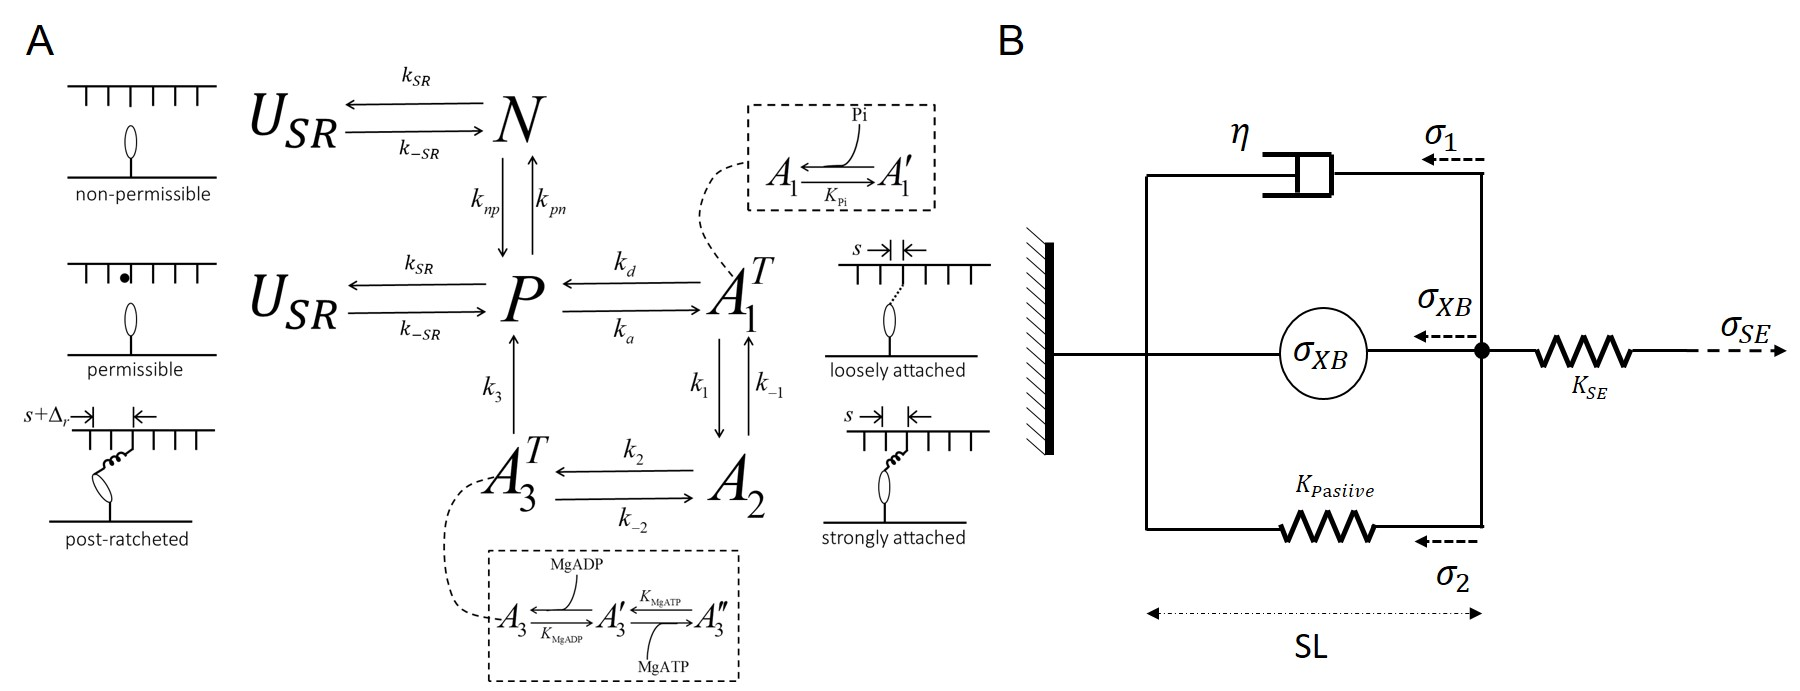
\includegraphics[width=1.0\linewidth]{FigS1.jpg}
\caption{Cardiomyocyte mechanics model. The multi-scale strain-dependent model for the cross-bridge cycle is illustrated in panel A. The integration of the cross-bridge force ($\sigma_{XB}$) into a model of muscle mechanics is illustrated in panel B.}
\label{fig:crossbridge}
\end{figure}

\subsection{Calcium activation:}
The calcium activation model is adopted from \cite{Campbell2018} model with minor modifications. The equations for calcium-mediated transition from the N to the P state are: 
\begin{eqnarray}
  J_{on}    &=& k_{on}  [{\rm Ca}^{2+} ]  N \left(1 + k_{coop} (1-N) \right) \nonumber \\ 
  J_{off} &=& k_{off}  P \left( 1 + k_{coop}  N \right)
\end{eqnarray}
The term $k_{coop} (1-N)$ is representative of cooperative activation.
The variable N represents the non-permissible state: 
\begin{eqnarray}
  P             &=& 1 - N - p_1^0 - p_2^0 - p_3^0 \nonumber \\
  \frac{dN}{dt} &=& -J_{on} + J_{off} 
\end{eqnarray}
where $P$ is the permissible (calcium-bound).

\subsection{Super-relaxed state:}
The Campbell et al. model for calcium activation includes a transition between a super-relaxed and not relaxed state.
\begin{eqnarray}
 U_{SR} \leftrightharpoons U_NR \nonumber \\
 U_{SR} + U_{NR} = 1
\end{eqnarray}
where the transition from super-relaxed ($U_{SR}$) to non-relaxed ($U_{NR}$) state is force-dependent:
\begin{equation}
  \frac{dU_{NR}}{dt} = k_{SR} \left( 1 + k_{force}  \sigma_{XB} \right)U_{SR} - k_{-SR}  U_{NR} \, .
\end{equation}
where $\sigma_{XB}$, is active contractile force and formulated in equation ~ \ref{eq:activeforce}. 

\subsection{Overlap function:}

Following \cite{Rice2008} the fractional overlap between thin and thick filament is represented as follows:
\[
  OV_{Z-axis} = min\left(L_{thick}/2,SL/2\right) \, ,
\]
where $OV_{Z-axis}$ is the overlap region closest to the Z-axis,
\[
  OV_{M-line} = max\left(SL/ 2 - (SL - L_{thin} \right), L_{bare}/2) \, ,	
\]
where $OV_{M-line}$ is the overlap region closest to the M-line. The length of overlap $LOV$ is computed as following:
\[
 LOV = OV_{Z-axis} - OV_{M-line}  \, .
\]
Using length of overlap LOV, fraction of thick filament overlap is computed as following:
\begin{eqnarray}
  OV_{thick} = 2 LOV / (L_{thick}- L_{bare} ) \, .
\end{eqnarray}
Here $SL$ is the length of sarcomere, $L_{thick}$ , $L_{thin}$ , $L_{bare}$ are the length of thick filament, bare region of the thick filament and, the length of the thin filament.

\begin{table}[ht]\centering
\small
\caption{Sarcomere overlap function parameters}\label{tab:6}
\begin{tabular}{l l l l}
\toprule
Parameter & Definition & Value and units & Parameter name in code \\
\midrule
$L_thin$      & thin filament length                 & 1200 nm & L\_thin  \\
$L_thick$     & thick filament length                & 1670 nm & L\_thick \\
$L_bare$      & bare length of the thick filament    & 100 nm  & L\_hbare \\
$OV_{Z-axis}$ &	overlap region closest to the Z-axis & nm      & sovr\_ze \\
$OV_{M-line}$ &	overlap region closest to the M-line & nm      & sovr\_cle \\
$LOV$	      & length of overlap                    & nm      & L\_sovr  \\
$OV_{thick}$  & fraction of thick filament overlap   & unitless  & N\_overlap \\

\bottomrule 
\end{tabular}
\end{table}

\subsection{Active and passive force:}

The active force generated by cross-bridges is computed from contributions from pre- and post-ratcheted states:
\begin{equation}\label{eq:activeforce}
  \sigma_{XB} (t) = OV_{thick} ( k_{stiff,1}  \left(p_2^2 + p_3^2 \right) + k_{stiff,2} \Delta r p_3^0 )
\end{equation}
where $k_{stiff,1}$ and $k_{stiff,2)}$ are stiffness constants, $\Delta r$ is the cross bridge strain associated with ratcheting deformation.
The full muscle model (Fig.~\ref{fig:crossbridge}) includes contributions from the active force generated by the cross-bridge mechanics, the viscous and passive forces associated with the muscle, $F_1$ and $F_2$, and a series element force $F_{SE}$. Overall force balance for the model yields
\begin{equation}\label{eq:totalforce}
  \sigma_{SE} (t) = \sigma_{XB} (t) + \sigma_1 (t) + \sigma_2 (t) \, .
\end{equation}
The stress contributed from the dashpot (viscous) is determined from the rate of change of sarcomere length.
\begin{equation}\label{eq:viscosity}
  \sigma_1 = \eta \frac{dSL}{dt} \, .
\end{equation}
The passive force $\sigma_2$ is a function of sarcomere length and is calculated 
\begin{equation}
  \sigma_2 (SL)= k_{passive}  \left(SL - SL_{rest} \right) + \sigma_{Passive_collagen} (SL)
\end{equation}
where $k_{passive}$ is the stiffness parameters for the passive force, $SL_{rest}$ is the sarcomere rest length, and the passive force exerted by collagen is adopted from \cite{Rice2008}.
\begin{eqnarray}
  \sigma_{Passive_collagen} (SL) = \left\{ \begin{array}{ll} 
    Pcon_{collagen} \left[ e^{PExp_{collagen}(SL - SL_{collagen})} -1 \right] &  if SL > SL_{collagen} \\ 
    0 & {\rm otherwise} \end{array} \right. \, .
\end{eqnarray}
where $Pcon_{collagen} = 0.01$ (unitless) is the scale factor for passive force contributed by collagen. 
$PExp_{collagen} = 70$ $\mu$m$^{-1}$ is a model parameter and $SL_{collagen} = 2.25$ $\mu$m is the minimum length threshold at which collagen starts to exert force on sarcomere.
 
\subsection{Model Parameters:}

Certain parameters from the cross-bridge and calcium-activation models of \cite{Tewari2016a,Tewari2016b} and \cite{Campbell2018} were re-estimated to match data from \cite{Janssen2002} on calcium transients and force-generation in isolated rat cardiac trabeculae. In brief, experiments were conducted at 37$^\circ$~C. Calcium transients (Fig.~\ref{fig:calcium}) were measured at different stimulation frequencies at fixed sarcomere length SL = 2.2 $\mu$m. Isometric tension time courses were measured at different stimulation frequencies and sarcomere lengths. Fig.~\ref{fig:calcium} shows data on peak developed tension ($T_{dev}$) as a function of $SL$ at stimulation frequency of 4~Hz; and data on relaxation time from peak to 50\% of peak tension ($RT50$); peak developed tension ($T_{dev}$) and time to peak tension ($TTP$) as function of $SL$.

Model simulations were fit to these data to estimate unknown parameters in the calcium activation and cross-bridge kinetics components of the model. Specifically, parameters adjusted to values different from those in the original publication are indicated below in Table~\ref{tab:7}.

\begin{figure}[ht]\centering
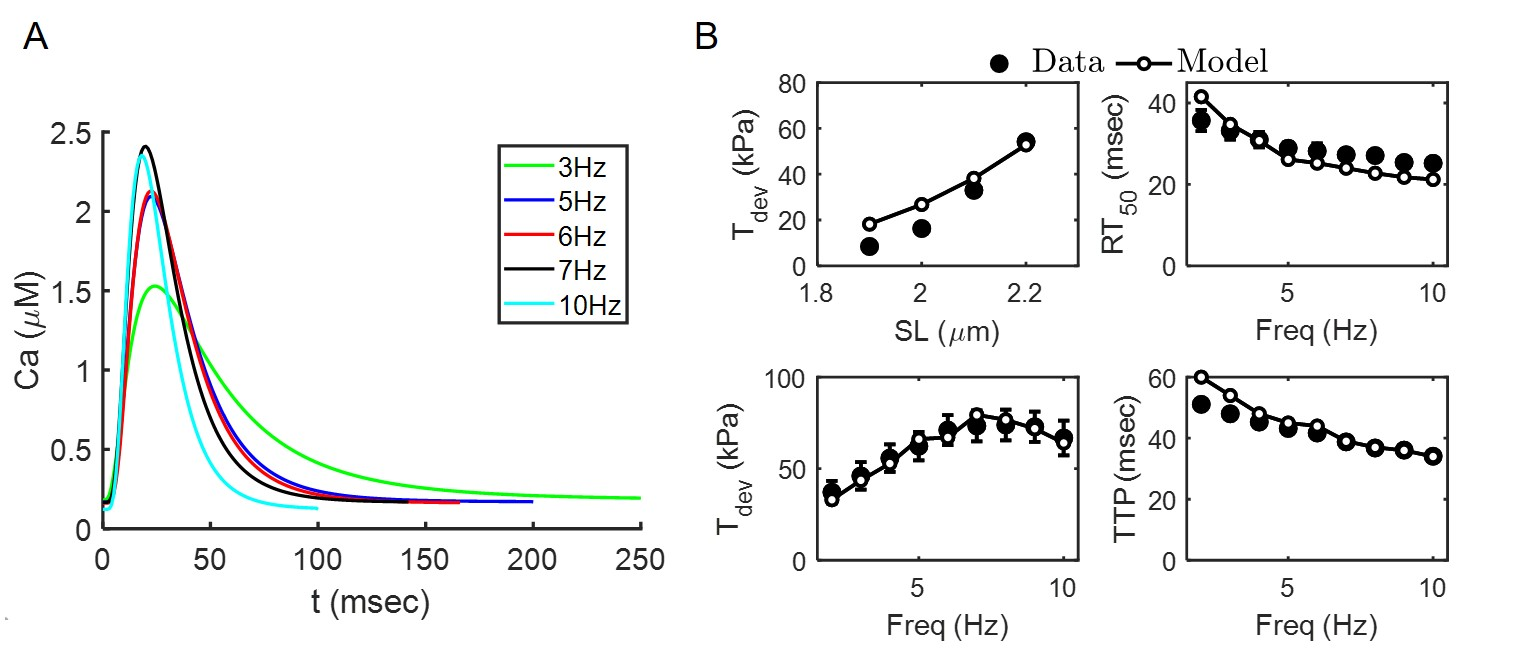
\includegraphics[width=1.0\linewidth]{CrossBridgeParaEstimate.jpg}
\caption{Crossbridge model parameters estimation. For $SL =1.9$~$\mu$m the $Ca_{50} = 5.89$ and Hill coefficient $n = 4.63$ and for $SL = 2.3$~$\mu$m the $Ca_{50} =6.001$ and Hill coefficient $n = 4.47$. Error bars shown in panel (B) represent standard error from the n = 9 data-set \cite{Janssen2002}.}
\label{fig:calcium}
\end{figure}

\begin{table}[!htb]
\centering
\small
\caption{Model parameters for cross bridge model }\label{tab:7}

\begin{supertabular}{p{1.4cm} p{4.4cm} p{1.8cm} p{2.0cm} p{2.0cm}}
\toprule
Parameter & Definition & Value and units & Parameter name in code & Reference \\
\midrule

$k_{stiff,1}$ & 
Stiffness constant due to myosin–actin interaction & 
13013 mmHg/$\mu$m & kstiff1 & 
Fit to data in Fig.~\ref{fig:calcium} \\

$k_{stiff,2}$ & 
Stiffness constant due to working stroke of XBs & 
341590 mmHg/$\mu$m  & kstiff2 &
Fit to data in Fig.~\ref{fig:calcium}  \\

$k_{passive}$ & Passive stiffness constant &
25 mmHg/$\mu$m & k\_passive &
Fit to data in Fig.~\ref{fig:calcium}  \\

$SL_{rest}$ & 
Sarcomere length at which passive force is zero  & 
1.8 $\mu$m & 
SL\_rest\_pas &
\cite{Campbell2018} \\

$\alpha_1$ & 
Strain-dependency parameter & 
10 $\mu$m$^{-1}$ & 
alpha1 &
\cite{Tewari2016b} \\

$\alpha_2$ & 
Strain-dependency parameter & 
9 $\mu$m$^{-1}$ & 
alpha2 &
\cite{Tewari2016b} \\

$\alpha_3$ & 
Strain-dependency parameter & 
5.93 $\mu$m$^{-2}$ & 
alpha3 &
Fit to data in Fig.~\ref{fig:calcium}  \\

$s_3$ & 
Strain-dependency parameter & 
$9.9 \times 10^{-3}$ $\mu$m &
s3 &
\cite{Tewari2016b} \\

$k_{coop}$ & 
Strength of thin filament cooperativity  & 
1.857 & 
K\_coop &
Fit to data in Fig.~\ref{fig:calcium}  \\

$k_{on}$ & 
Rate constant of Ca binding to troponin C & 
101.2~$\mu$M$^{-1}\cdot$s$^{-1}$ & 
k\_on &
Fit to data in Fig.~\ref{fig:calcium}  \\

$k_{off}$ & 
 Rate constant of Ca unbinding from troponin C  & 
101.2~s$^{-1}$ & 
k\_off &
Fit to data in Fig.~\ref{fig:calcium}  \\

$k_{force}$ & 
 Force-dependent  rate constant of super relax transition  & 
  $1.169 \times 10^{-3}$ N$^{-1}\cdot$m$^{-2}$ & kforce &
Fit to data in Fig.~\ref{fig:calcium}  \\

$k_{SR}$ & 
Rate constant of force-dependent super relax transition  & 
14.44~s$^{-1}$ & 
ksr &
Fit to data in Fig.~\ref{fig:calcium}  \\

$k_{-SR}$ & 
Rate constant of force-dependent super relax transition  & 
50.03~s$^{-1}$ & 
kmsr &
Fit to data in Fig.~\ref{fig:calcium}  \\

$k_{MgATP}$ & 
[MgATP] dissociation constant  & 
489.7 $\mu$M &
K\_T &
\cite{Tewari2016b} \\

$k_{MgADP}$ & 
[MgADP] dissociation constant  & 
194.0 $\mu$M &
K\_D &
\cite{Tewari2016b} \\

$k_{Pi}$ & 
[Pi] dissociation constant  & 
4.0 mM &
K\_Pi &
\cite{Tewari2016b} \\

$k_a$ & 
Myosin–actin rate of attachment  & 
559.6~s$^{-1}$ & 
ka &
Fit to data in Fig.~\ref{fig:calcium}  \\

$k_d$ & 
Myosin–actin rate of un-attachment  & 
304.7~s$^{-1}$ & 
kd &
Fit to data in Fig.~\ref{fig:calcium}  \\

$k_1$ & 
 Transition rate constant  & 
112.4~s$^{-1}$ & 
k1 &
Fit to data in Fig.~\ref{fig:calcium}  \\

$k_{-1}$ & 
Rate of strongly-bound to weakly-bound transition  & 
21.30~s$^{-1}$ & 
km1 & 
\cite{Tewari2016b} \\

$k_2$ & 
Rate of ratcheting  & 
811.7~s$^{-1}$ & 
k2 & 
\cite{Tewari2016b} \\

$k_{-2}$ & 
Reverse ratcheting rate  & 
43.25~s$^{-1}$ & 
km2 & 
\cite{Tewari2016b} \\

$k_3$ & 
 Myosin–actin  detachment rate  & 
144.6~s$^{-1}$ & 
k3 &
Fit to data in Fig.~\ref{fig:calcium}  \\

\bottomrule 
\end{supertabular}
\end{table}

\section{Heart Model}

\subsection{Model Variables and Equations:}

A modified version of the \cite{Lumens2009} TriSeg model is used to simulate left- and right-ventricular mechanics, based on the implementation of \cite{Tewari2016b}. Tension development in each of the left-ventricular free wall, septum, and right-ventricular free wall is simulated using a cell mechanics model to represent each of these segments. From Eq. (\ref{eq:viscosity}) the rates of change of sarcomere length in these three segments is given by

\begin{eqnarray}\label{eq:sarcomererate}
\frac{dSL_{RV}}{dt} &=& \frac{\sigma_{SE,RV} - \sigma_{2}(SL_{RV}) - \lambda_{XB}\sigma_{XB,RV}(t)}{\eta}     \nonumber \\
\frac{dSL_{LV}}{dt} &=& \frac{\sigma_{SE,LV} - \sigma_{2}(SL_{LV}) - \lambda_{XB}\sigma_{XB,LV}(t)}{\eta}     \nonumber \\
\frac{dSL_{SEP}}{dt} &=& \frac{\sigma_{SE,SEP} - \sigma_{2}(SL_{SEP}) - \lambda_{XB}\sigma_{XB,SEP}(t)}{\eta}
\end{eqnarray}
where the parameter $\lambda_{XB}$ is a scalar used to account for differences in force generation in vivo versus in vitro. (The value value $\lambda_{XB}$ = 1.4, determined by \cite{Tewari2016b} accounts for slightly lower force generation in vitro versus in vivo.)

The $SL$ and $\frac{dSL}{dt}$ computed from Eq.~(\ref{eq:sarcomererate}) are used in Eqs.~(\ref{eq:equations_crossbridge}) which govern cross-bridge dynamics in each segment. The dynamical state of the cross-bridge model in each segment, in turn, appears in Eq.~(\ref{eq:sarcomererate}), which governs $SL(t)$ for each segment.

The series element elastic force for each segment is computed to be proportional to the difference between the sarcomere length and the sarcomere length calculated from natural myofiber strain:

\begin{eqnarray}\label{eq:TriSeg1}
\sigma_{SE,RV} &=& K_{SE}(SL_{0,RV} - SL_{RV})   \nonumber \\
\sigma_{SE,LV} &=& K_{SE}(SL_{0,LV} - SL_{LV})   \nonumber \\
\sigma_{SE,SEP} &=& K_{SE}(SL_{0,SEP} - SL_{SEP}) \nonumber 
\end{eqnarray}
where
\begin{eqnarray}\label{eq:TriSeg2}
SL_{0,\#} &=& SL_{ref} exp(\epsilon_{f,\#}) )   \nonumber \\
\epsilon_{f,\#} &=& \frac{1}{2} ln (\frac{A_{m,\#}}{A_{m,ref,\#}}) - \frac{1}{12} z_{\#}^{2} - 0.019 z_{\#}^{4}  \nonumber \\
z_{\#} &=& \frac{3C_{m,\#}V_{W,\#}}{2A_{m,\#}} \nonumber \\
V_{m,\#} &=& \frac{\pi}{6} x_{m,\#} (x_{m,\#}^2 + 3y_{m}^{2}) \nonumber \\
A_{m,\#} &=& \pi(x_{m,\#}^2 + y_{m}^{2}) \nonumber \\
C_{m,\#} &=& \frac{2x_{m,\#}}{x_{m,\#}^{2}+y_{m}^{2}} \, . \nonumber
\end{eqnarray}
Here $A_{m,\#}$ the midwall surface area of segment \#, $A_{m,ref,\#}$ is a reference midwall surface area, $C_{m,\#}$ is the curvature of the midwall surface, $V_{w,\#}$ is the wall volume of wall segment i, $V_{m,\#}$ is the midwall volume, and $x_{m,\#}$ and $y_{m}$ determine the geometry of the LV and RV cavity (see \cite{Lumens2009}). The four variables of the TriSeg heart model, $x_{m,RV}$ , $x_{m,LV}$, $x_{m,SEP}$, and $y_{m}$ that determine the geometry of the ventricular cavities, are listed in Table~\ref{tab:8}. 

\begin{table}[ht]\centering
\small
\caption{State variables in TriSeg (Heart) model}\label{tab:8}
\begin{tabular}{l l l l}
\toprule
State Variable  & Definition & Units & Variable name in code \\
\midrule
{x}$_m,RV$ & \begin{tabular}{l}Maximal axial distance \\ from RV midwall surface to origin\end{tabular} & cm & Xm\_RV \\
{x}$_m,LV$ & \begin{tabular}{l}Maximal axial distance \\ from LV midwall surface to origin\end{tabular} & cm  & Xm\_LV \\
{x}$_m,SEP$ & \begin{tabular}{l}Maximal axial distance \\ from SEP midwall surface to origin\end{tabular} & cm  & Xm\_SEP \\
{y}$_m$  & Radius of midwall junction circle & cm  & ym \\
\bottomrule
\end{tabular}
\end{table}

For given wall volumes and ventricular volumes, the geometry of the heart is solved such that equilibrium of radial and axial tensile forces is achieved at the junction margin (i.e., where the three wall segments meet forming ventricular cavities).

Tension in the midwall of each segment is calculated as a function of stress: 

\begin{equation}
    T_{m,\#} = \frac {V_{W,\#} \sigma_{SE,\#}}{2A_{m,\#}} 
    \left(1+\frac{z^{2}}{3}+\frac{z^{4}}{5}\right)
\end{equation}

Axial and radial components of the tension are computed 

\begin{eqnarray}
 T_{x,\#} = T_{m,\#} \frac{2x_{m,\#}y_{m}}{x_{m,\#}^{2}+y_{m}^{2}} \nonumber \\
 T_{y,\#} = T_{m,\#} \frac{-x_{m,\#}^{2}+y_{m}^{2}}{x_{m,\#}^{2}+y_{m}^{2}}
\end{eqnarray}
   
The four unknowns of the model---$x_{m,RV}$ , $x_{m,LV}$, $x_{m,SEP}$, and $y_{m}$---are determined by satisfying the relations
\begin{eqnarray}
  & V_{m,LV} = -V_{LV} - \frac{1}{2} V_{w,LV} - \frac{1}{2} V_{w,SEP} + V_{m,SEP} \nonumber \\
  & V_{m,RV} = +V_{RV} - \frac{1}{2} V_{w,RV} - \frac{1}{2} V_{w,SEP} - V_{m,SEP} \nonumber \\
  & T_{x,RV} + T_{x,LV} + T_{x,SEP} = 0 \nonumber \\
  & T_{y,RV} + T_{y,LV} + T_{y,SEP} = 0 \nonumber \, .
\end{eqnarray}
Transmural pressures are computed
\begin{equation}
    P_{trans,\#} = \frac{2T_{x,\#}}{y_{m}}
\end{equation}
and the pressures in the cavities are computed
\begin{eqnarray}
P_{LV} &=& - P_{trans,LV} \nonumber \\
P_{RV} &=& + P_{trans,RV} \nonumber \, .
\end{eqnarray}
\subsection{Model Parameters}

Parameters defining the mass and geometry of the heart are identified from data on individual animals are defined in Table~\ref{tab:9}.

\begin{table}[ht]\centering
\small
\caption{Parameters in TriSeg (Heart) model}\label{tab:9}
\begin{tabular}{l l l l}
\toprule
Parameter & Definition & Value and Units & Variable name in code \\
\midrule
$V_{w,LV}$ & LV wall volume &\begin{tabular}{l}input\\(experimental data), mL \end{tabular} & Vw\_LV \\
$V_{w,SEP}$ & Septal wall volume &\begin{tabular}{l}input\\(experimental data), mL \end{tabular} & Vw\_SEP \\
$V_{w,RV}$ & RV wall volume &\begin{tabular}{l}input\\(experimental data), mL \end{tabular} & Vw\_RV \\
$A_{m,ref}^{LW}$ &\begin{tabular}{l}
 LV midwall reference\\surface area
\end{tabular} & adjustable, cm$^{2}$ & Amref\_LV \\
$A_{m,ref}^{SEP}$ &\begin{tabular}{l}
 Septal midwall reference\\surface area
\end{tabular} & adjustable, cm$^{2}$ & Amref\_SEP \\
$A_{m,ref}^{RW}$ &\begin{tabular}{l} RV midwall reference\\surface area
\end{tabular} & adjustable, cm$^{2}$  & Amref\_RV \\
$K_{SE}$ & Stiffness of series element & 50000 mmHg/$\mu$m  & Kse \\
$\eta$  & Viscosity coefficient of myofibers & 1 mmHg$\cdot$sec$\cdot \mu$m$^{-1}$  & eta \\
\bottomrule
\end{tabular}
\end{table}

\section{Lumped-Parameter Cardiovascular Systems Model}

\subsection{Model Variables and Equations:}

The lumped-parameter model illustrated in Fig.~\ref{fig:CVS} is used to simulate pressures and flows in the systemic and pulmonary circuits. This simple lumped model invokes eight parameters representing: pulmonary resistance $R_{pul}$, pulmonary arterial and venous compliances $C_{PA}$ and $C_{PV}$, systemic arterials resistances $R_{Ao}$ and $R_{sys}$, systemic arterial compliance $C_{SA}$, and systemic venous compliance $C_{SV}$, systemic arterial resistance and aortic compliance $C_{Ao}$. 
\begin{figure}[ht]\centering
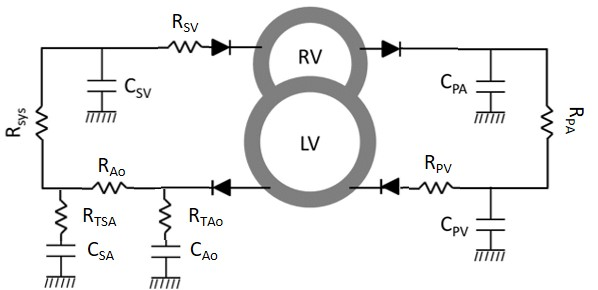
\includegraphics[width=0.65\linewidth]{CVS.jpg}
\caption{Cardiovascular system (CVS) diagram. Adopted from Tewari et al. \cite{Tewari2016a,Tewari2016b}. $C_{PA}$, $C_{PV}$, $C_{SA}$, $C_{Ao}$, and $C_{SV}$ represent lumped compliances of pulmonary arteries, pulmonary veins, systemic arteries, aorta, and systemic veins. $R_{pul}$, $R_{sys}$, and $R_{Ao}$ represent vascular resistances. The lumped-parameter representations of the systemic and pulmonary circuits are coupled to the TriSeg heart model of \cite{Lumens2009}, described below.}\label{fig:CVS}
\end{figure}

Flow through a resistive element is calculated
\begin{equation}\label{eq:flow}
    q =\frac{P_{1} - P_{2}}{R}
\end{equation}
where $P_{1} - P_{2}$ is the pressure drop across the element, and R is the resistance. Pressure in a compliant/capacitive element is governed by
\begin{equation}\label{eq:dPdT}
    \frac{dP}{dt} =\frac{F_{in} - F_{out}}{C} 
\end{equation}
where $F_{in} - F_{out}$ is the rate of change of blood volume in the element.
Table~\ref{tab:10} lists the variables of the cardiovascular systems model. These variables and Eqs. ~\ref{eq:flow} and ~\ref{eq:dPdT} are invoked in the MATLAB code {\em Cardiovascularmechancis.m}.

\begin{table}[ht]\centering
\small
\caption{Variables used in lumped-parameter cardiovascular model}\label{tab:10}
\begin{tabular}{l l l l}
\toprule
Parameter & Definition & Units used in code & Variable name in code \\
\midrule
\multicolumn{4}{l}{\em Cardiovascular system model state variables} \\
$V_{LV}$ & Left ventricle volume & mL & V\_LV \\
$V_{RV}$ & Right ventricle volume & mL & V\_RV \\
$V_{SV}$ & Volume of systemic vein & mL & V\_SV \\
$V_{PV}$ & Volume of pulmonary vein & mL & V\_PV \\
$V_{SA}$ & Volume of systemic artery & mL & V\_SA \\
$V_{PA}$ & Volume of pulmonary artery & mL & V\_PA \\
$V_{Ao}$ & Volume of aorta & mL & V\_Ao \\

\multicolumn{4}{l}{\em Pressures computed from volume state variables} \\
$P_{SV}$ & Systemic venous pressure & mmHg & P\_SV \\
$P_{PV}$ & Pulmonary venous pressure & mmHg & P\_PV \\
$P_{PA}$ & Pulmonary arterial pressure & mmHg & P\_PA \\
$P_{Ao}$ & Aortic pressure (proximal to TAC) & mmHg & P\_Ao \\
$P_{SA}$ & Systemic arterial pressure (distal to TAC) & mmHg & P\_SA \\

\bottomrule
\end{tabular}
\end{table}

\subsection{Identification of Model Parameters:}

Table~\ref{tab:11} lists the parameters used in the lumped circulatory model.

\begin{table}[ht]\centering
\small
\caption{Parameter used in the CVS model}\label{tab:11}
\begin{tabular}{l l l l}
\toprule
Parameter & Definition & Value and Units & \begin{tabular}{l}Variable name\\
in code
\end{tabular} \\
\midrule
$C_{Ao}$ & Proximal aortic compliance & 0.0022045 mL$\cdot$mmHg$^{-1}$ & C\_Ao \\
$C_{SA}$ & Systemic arterial compliance & 0.0077157  mL$\cdot$mmHg$^{-1}$ & C\_SA \\
$C_{SV}$ & Systemic venous compliance & 2.5 mL$\cdot$mmHg$^{-1}$ & C\_SV \\
$C_{PA}$ & Pulmonary arterial compliance & 0.013778 mL$\cdot$mmHg$^{-1}$ & C\_PA \\
$C_{PV}$ & Pulmonary venous compliance & 0.25  mL$\cdot$mmHg$^{-1}$ & C\_PV \\
$R_{Ao}$ & Proximal aortic resistance & 2.5 mmHg$\cdot$sec$\cdot$ mL$^{-1}$   & R\_Ao \\
$R_{sys}$ & Systemic vasculature resistance & adjustable, mmHg$\cdot$sec$\cdot$ mL$^{-1}$    & R\_sys \\
$R_{SV}$  & Systemic veins resistance & 0.25 mmHg$\cdot$sec$\cdot$ mL$^{-1}$    & R\_SV \\
$R_{TAo}$ & Transmural aortic resistance & 0.5 mmHg$\cdot$sec$\cdot$ mL$^{-1}$    & R\_tAo \\
$R_{TSA}$ & Transmural systemic artery resistance & 4 mmHg$\cdot$sec$\cdot$ mL$^{-1}$    & R\_tSA \\
$R_{PA}$  & Pulmonary vasculature resistance & 7.58 mmHg$\cdot$sec$\cdot$ mL$^{-1}$   & R\_PA \\
$R_{PV}$ & Pulmonary veins resistance & 0.25 mmHg$\cdot$sec$\cdot$ mL$^{-1}$    & R\_PV \\
$R_{VLV}$ & Valve resistance & 0.05 mmHg$\cdot$sec$\cdot$ mL$^{-1}$    & R\_VLV \\
$R_{TAC}$  & Resistance of TAC & adjustable, mmHg$\cdot$sec$\cdot$ mL$^{-1}$   & R\_TAC \\

\bottomrule
\end{tabular}
\end{table}

The systemic compliances ($C_{SA}$,$C_{Ao}$, $C_{SV}$) are fixed to produce a pulse pressure of roughly 33 mmHg for simulations of sham control rats. The pulmonary compliance ($C_{PA}$, $C_{PV}$) are fixed to roughly have the target value of 12 mmHg for the pulmonary pulse pressure. The resistance $R_{Ao}$ is arbitrarily set to have a small pressure drop of 4 mmHg between the aorta and systemic arteries for cardiac output of the mean value of 95 mL per min. The systemic venous resistance $R_{SV}$ is set so that the mean pressure in the systemic veins for sham control rats is 3 mmHg. The pulmonary resistances $R_{PA}$ and $R_{PV}$ are set to give a mean pulmonary arterial pressure of 21 mmHg and pulmonary venous pressure of 9 mmHg in the sham control rats.

The two parameters in the circulation model that are adjusted to match measured data on individual TAC and sham rats are $R_{TAC}$ and $R_{sys}$. The resistance $R_{TAC}$ represents the resistance across the transverse aortic constriction (TAC), and is set to zero in sham-operated rats. In TAC rats, the value of this resistance is obtained based on the pressure gradient across the TAC constriction estimated from ultrasound measurements of the velocity gradient. The pressure drop across the constriction is computed $\Delta P_{TAC} = \frac{1}{2} \rho (V_{2}^{2} - V_{1}^{2})$, where $V_{1}$ and $V_{2}$ are the velocities on either side of the TAC constriction. Given an estimated pressure drop the resistance is computed $R_{TAC} = \frac{\Delta P_{TAC}}{CO}$, where CO is the cardiac output. The systemic resistance $R_{sys}$ is adjusted so that the mean arterial pressure (MAP) is maintained at 93.3 mmHg. (Model fitting procedures are detailed below in Section~\ref{sec:ModelFits}.)

\section{Model fits and predictions associated with individual rats}\label{sec:ModelFits}

\subsection{Summary:}

The cardiac energy metabolism and the whole-body cardiovascular mechanics model (which includes the heart model) are implemented as separate modules. These models are matched to data on an individual animal basis. The cardiac energetics model takes as an input the myocardial ATP consumption rate, the measured metabolite pools levels, and the measured mitochondrial ATP synthesis capacity, and outputs the cytoplasm concentrations of phosphate metabolites. The cardiac mechanics code takes as an input the cytoplasmic concentrations of phosphate metabolites (namely, ATP, ADP, and Pi) and computes as an output the ventricular end-systolic and end-diastolic volumes and arterial pressures to compare to measured data, and the myocardial ATP hydrolysis rate to use in the energetics module. The energetics and mechanics models are iteratively run until they simultaneously converge to a steady state at fit the target cardiovascular data.

\begin{table}[!htb]
\centering
\small
\caption{Input arguments and adjustable parameters for cardiovascular mechanics model}\label{tab:12}

\begin{supertabular}{p{1.8cm} p{1.4cm} p{3.0cm} p{1.8cm} p{3.6cm}}
\toprule
Parameter & Variable name in code & Definition & Units used in code & Values  \\
\midrule
HR & HR & Heart rate & bpm &  318.6--367 for sham 294--349 for TAC. Set to measured value \\

Vw,LV & Vw\_LV & LV wall volume & mL &  0.564--0.853 for sham 
0.863--1.22 for TAC. Set as 2/3 of measured LV volume \\

Vw,SEP & Vw\_SEP & Septal wall volume & mL &  0.2821--0.4266 for sham 
0.431--0.61 for TAC. Set as 1/3 of measured LV volume \\

Vw,RV & Vw\_RV & RV wall volume & mL &  0.282--0.373 for sham
0.249--0.605 for TAC. Set as measured RV free wall volume \\

$A_{m,ref}^{LW}$ & Amref\_LV & 
 LV midwall reference surface area
 & cm$^{2}$ &   1.6865--2.465 for SHAM
 2.299--2.966 for TAC.
 Adjusted to fit data
 \\

$A_{m,ref}^{SEP}$ & Amref\_SEP & 
 Septal midwall reference surface area
 & cm$^{2}$ &  1.055--1.487 for sham
1.299--1.620 for TAC.
 Adjusted to fit data
 \\

$A_{m,ref}^{RW}$ & Amref\_RV & 
 RV midwall reference surface area
 & cm$^{2}$ &  2.629--3.612 for sham
3.135--5.538 for TAC.
 Adjusted to fit data
 \\

$k_{force}$ & k\_force & Model parameter for force dependent super relax transition   & 
N$^{-1}$ m$^{2}$ &  (0.905--3.312)$\times 10^{-3}$ for sham
(1.464--3.783)$\times 10^{-3}$ for TAC. 
 Adjusted to fit data
 \\

$k_{SR}$ & ksr & On rate  constant for super relax state
& s$^{-1}$ &  9.021--33.013 for sham
14.598--37.708 for TAC.
 Adjusted to fit data
 \\

$R_{sys}$ & R\_sys & Systemic vasculature resistance
 & mmHg$\cdot$sec$\cdot$ mL$^{-1}$  &  38.071--71.886 for sham
50.577--125.33 for TAC.
 Adjusted to fit data
 \\

$R_{TAC}$ & R\_TAC & resistance of TAC & mmHg$\cdot$sec$\cdot$ mL$^{-1}$  &  0 for sham
7.11--22.25 for TAC.
 Adjusted to fit data
 \\

MgATP\_cyto-plasm
 & MgATP & cytosolic [MgATP] & mmole$\cdot$(L cytosol water)$^{-1}$
 &  7.214--9.439 for sham
4.938--9.063 for TAC .
Predicted from energetics model 
 \\

MgADP\_cyto-plasm
  & MgADP & cytosolic [MgADP] & mmole$\cdot$(L cytosol water)$^{-1}$
  &  0.047--0.06 for sham
0.027--0.055 for TAC.
Predicted from energetics model 
 \\

Pi\_cyto-plasm
  & Pi & cytosolic total [Pi] & mmole$\cdot$(L cytosol water)$^{-1}$
 &  0.740--2.197 for sham
1.922--2.798 for TAC.
Predicted from energetics model \\

\bottomrule
\end{supertabular}
\end{table}

\subsection{Relationship between cross-bridge cycle and ATP hydrolysis rates:}

The relationship between cross-bridge cycle rate and J\_ATP, the rate myocardial oxygen consumption rate, is based on matching the myocardial oxygen consumption rate predicted by the model to that observed for the working rat heart. \cite{Duevelleroy1976} report a mean oxygen consumption rate of approximately $MVO2 = 0.31$ mL$\cdot$(min$\cdot$g)$^{-1}$ for work rates corresponding to resting state in blood perfused working hearts. Using a myocardial cell density (in terms of cardiomyocyte volume per unit mass of myocardium) of $\rho_{cell} = 0.694$ mL$\cdot$g$^{-1}$ and assuming a P/O2 ratio (moles of ATP synthesized per mole of O2 consumed) of 4.5 \cite{Wu2008}, we estimate a resting ATP hydrolysis rate of $1.30$ mmol$\cdot$(sec$\cdot$L cell)$^{-1}$. (This value is approximately 2.5 times higher than the estimated resting ATP hydrolysis rate of to $0.547$ mmol$\cdot$(sec$\cdot$L cell)$^{-1}$ for human myocardium \cite{Gao2019}.) 

Simulations of the cardiovascular mechanics model predict an average cross-bridge cycling rate of 5.03 sec$^{-1}$ for the mean sham-operated control rat. Assuming a fixed proportionality between cross-bridge cycling rate and myocardial ATP hydrolysis rate, yields a constant of proportionality of 
\begin{eqnarray}
 & & {\rm ATP\, hydrolysis\, rate (mmol\cdot(sec \cdot L \, cell)^{-1})}  = \nonumber \\
 & & {\rm 0.258 \, (mmol \cdot (L \, cell)^{-1}) \times crossbridge \, cycling \,rate \, (sec^{-1}) } \, .
\end{eqnarray}
If we assume that roughly 3/4 of the ATP consumed by the cardiomyocyte is consumed by the myosin ATPase, we estimate from this constant of proportionality the density of cross-bridge-forming units in a cardiomyocyte to be roughly 0.34 mmol per liter of cell. This density has been independently estimated to be 0.25 mmol per liter of cell for skeletal myocytes (\cite{Barclay2010}).

\subsection{Fitting data on individual rats:}

The full set of adjustable parameters invoked in the cardiovascular systems model is listed in Table 12. Certain adjustable parameters are set based on direct measurements and others are adjusted so that simulation outputs match measured data. Seven parameter values---$A_{m,ref}^{LW"}$ , $A_{m,ref} ^{SEP}$ , $A_{m,ref}^{RW}$ , $k_{force}$, $k_{SR}$, $R_{sys}$, $R_{TAC}$---are adjusted to fit model predictions to data from individual animals on end-systolic and end-diastolic volumes and estimated pressure drop across the aortic constriction in TAC animals, and to simultaneously maintain a fixed mean arterial pressure of 93.3 mmHg, to maintain end-diastolic sarcomere lengths in the LV, septum, and RV of 2.2 $\mu$m. 

Ranges of estimated values of are listed in Table~\ref{tab:12}. Values of anatomical/geometric parameters representing heart masses and reference areas are higher in TAC rats than in sham control rats, reflecting hypertrophic remodeling.
The parameters $k_{force}$ and $k_{SR}$ govern the transition out of the inaccessible super-relaxed state in the calcium-activation model. Increased in the values of these parameters represent increased levels of phosphorylation of myosin binding protein C. Thus, the higher values of these parameters in TAC compared to sham animals represent a prediction that phosphorylation of this protein is increased in the TAC animals.

Simulations of TAC rats consistently show lower ATP, ADP, and CrP, reflecting reductions in the total adenine nucleotide and creatine pools. (See below.) Lower ADP levels require a compensatory increase in inorganic phosphate to maintain ATP synthesis. 

The ranges of values of cross-bridge cycle rate, ATP hydrolysis rate, and end-systolic and end-diastolic volumes are listed in Table~\ref{tab:13}. 



\begin{table}[ht]\centering
\small
\caption{Output arguments for cardiovascular mechanic model}\label{tab:13}
\begin{supertabular}{p{2.5cm} p{3.0cm} p{2.5cm} p{3.4cm}}
\toprule
Variable & Definition & Units used in code & Values \\
\midrule

rate\_of\_XB\_turn-over\_ave 
& Cross bridge cycling rate & sec$^{-1}$ & 
3.5874--5.3658 for sham
2.606--5.4381 for TAC
 \\
 
x\_ATPase & ATP hydrolysis rate & mmol$\cdot$(sec$\cdot$L$\cdot$cell)$^{-1}$ & 
0.9301--1.392 for sham
0.6758--1.410 for TAC
\\

EDLV & End diastolic left ventricular volume
& mL & 
0.303--0.547 for sham
0.407--0.650 for TAC
 \\
 
ESLV & 
End systolic left ventricular volume
 & mL & 
  0.093 -- 0.232 for sham
0.138 -- 0.423 for TAC
 \\
 
MAP & Mean arterial pressure & mmHg & 93.3 for both TAC and sham \\

\bottomrule
\end{supertabular}
\end{table}

The set of input parameters invoked in the cardiovascular systems model is listed in Table~\ref{tab:3}. The input parameters TAN, CRtot, and Ox\_capacity are all measured for each individual rat. The ATP hydrolysis rate ($x_{ATPase}$) is predicted by the mechanics model (see above). The relationships between metabolite pools from \cite{Gao2019} are used to estimate the total exchangeable phosphate (TEP):
\[
  {\rm TEP} = P_{0} - p ((A_{0} - {\rm TAN} )/ a)
\]
where, $P_{0}= 35.446$ mmol$\cdot$(L cell)$^{-1}$,  $A_{0} = 10.26$ mmol$\cdot$(L cell)$^{-1}$, are reference TEP and TAN values, $p = 0.283$mmol$\cdot$(L cell$\cdot$year)$^{-1}$  and $a = 0.082$ mmol$\cdot$(L cell$\cdot$year)$^{-1}$ are the slopes of the relationships between mean TEP and mean TAN and age in humans, respectively. 

Output arguments from the energetics model, including the metabolite levels used in the mechanics model, are listed in Table~\ref{tab:4}.

\subsection{Predictions associated with changing metabolic/energetic parameterization:}

The predictions illustrated in Fig. 9 of \cite{Lopez2020} are made by replacing the parameters representing the metabolic state of sham control rats with those representing TAC rats and by replacing the parameters representing the metabolic state of TAC rats with those representing sham control rats. 

For predictions of how mechanical function in sham rats changes when the metabolic profile is replaced with that of the average TAC rat (Fig. 9A - 9B \cite{Lopez2020}), the input metabolic parameters are set to:

\begin{eqnarray}
  {\rm TAN}   &=& 0.006976 \,  {\rm M} \nonumber \\
  {\rm CRtot} &=& 0.02303 \,  {\rm M} \nonumber \\
  {\rm TEP}   &=& 0.02411 \,  {\rm M} \nonumber \\
  {\rm Ox\_capacity} &=& 0.7482 \,  {\rm (unitless)} \nonumber
\end{eqnarray}

Note that the above average TAC rat metabolite profile are based on $n = 10$ TAC rats. (TAC \#7 is excluded for reasons described in \cite{Lopez2020}.)

Given these values specifying the metabolic model, the blood volume, $k_{force}$, and $k_{SR}$ are increased so that the model-predicted mean arterial pressure was 93.3~mmHg. In other words, it is assumed that baseline cardiac output and system pressure are maintained at the original physiological levels via compensatory increases in preload and myosin binding protein C phosphorylation. To obtain the model predictions in Lopez et al. first the $k_{force}$ and $k_{SR}$ are proportionately increased to compensate for the metabolic dysfunction. If it is not possible to restore mean arterial pressure to the physiological level with that change alone, blood volume is increased until the mean pressure of 93.3~mmHg is reached.

For predictions of how mechanical function in TAC rats changes when the metabolic profile is replaced with that of the average sham rat (Fig. 9C - 9D), the input metabolic parameters are set to:
\begin{eqnarray}
  {\rm TAN}   &=& 0.007624 \,  {\rm M} \nonumber \\
  {\rm CRtot} &=& 0.03027 \, {\rm M} \nonumber \\ 
  {\rm TEP}   &=& 0.02635 \, {\rm M} \nonumber \\
  {\rm Ox\_capacity} &=& 1 \, {\rm (unitless)} \nonumber
\end{eqnarray}

Given these values specifying the metabolic model, the blood volume, $k_{force}$, and $k_{SR}$ , and $R_{sys}$ are adjusted so that the model-predicted mean arterial pressure is 93.3 mmHg and the predicted end-diastolic volume with mean sham metabolic parameters is equal to that of the original TAC rat. In other words, it was assumed that baseline system pressure and diastolic filling level are maintained at the original physiological levels via compensatory reduction in preload, myosin binding protein C phosphorylation, and systemic resistance. 

\section{Running the model}

\subsection{Summary of codes}

The simulation package consists of 5 MATLAB files:
\begin{enumerate}
    \item CardiovascualarMechanics.m
    \item dXdT\_CardiovascularMechanics.m
    \item EnergeticsModelScript.m
    \item dXdT\_energetics.m
    \item TrisegEquations.m
\end{enumerate}

Values of all adjustable parameters are stored in spreadsheet files ``Adjustable\_paramaters\_table\_rest.xlsx'' for the baseline simulations and ``Adjustable\_parameters\_table\_SWAP.xlsx'' for simulations with replaced metabolic parameters.

The {\em CardiovascularMechanics.m} function is the main driver to run the mechanics model for a given animal. For instance, assigning the variable ``rat\_number'' to 1 will execute simulations for SHAM rat number 1. Executing the script will load the parameters associated with this animal, run the cardiovascular systems model for 120 heart beats to attain a periodic steady state, and then plot the predicted left ventricular pressure, aortic pressure, and arterial pressure along with the left-ventricular pressure volume loop for this individual animal. The target end-diastolic and end-systolic volumes and the pres-sure drop across the TAC will be indicated by dashed lines in the figures. The model will compute the predicted cross-bridge cycling rate in the LV free wall and the associated ATP hydrolysis rate.

The energetics model for a given animal is called within the cardiovascular model. Executing this script will read the metabolic/energetic parameters associated with this animal and run the model to calculate the cytosolic metabolite levels. Note the ATPase hydrolysis rate for steady state is pre-identified and is listed in column 9 of the input adjustable\_parameters\_table\_rest.xlsx. 

The numbering for rats in the input ``data1.xlsx'' file is as follows: the first 8 rats are SHAM rats and rat number 9 is the mean sham rat; rat number 10 to 19 are the TAC rats (TAC rat\# 7 is excluded). Therefore the first TAC rat is rat number 10 in the simulations. For example, to simulate the model for TAC rat \#1 we need assign number 10 to the variable ``rat\_numbers = 10'' in the {\em CardiovascularMehanics.m} and run the code. 

The model will generate output shown below in Fig.~\ref{fig:output}. 

\begin{figure}[ht]\centering
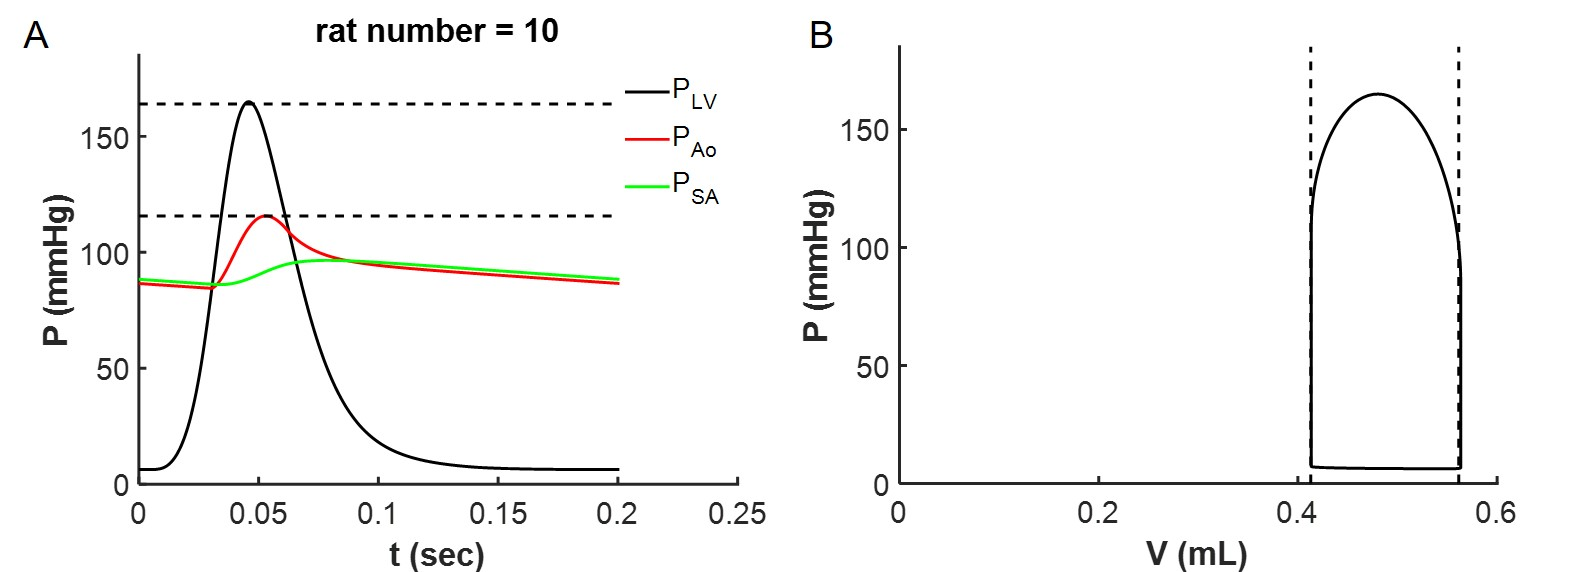
\includegraphics[width=1.0\linewidth]{FigS4.jpg}
\caption{Model output for TAC rat \#1.}\label{fig:output}
\end{figure}

In addition to the plots illustrated above, the running the model for this individual animal results in a predicted ATP hydrolysis rate of 0.675 mmole$\cdot$sec$^{-1}\cdot$(L cell)$^{-1}$. Note that the input ATP hydrolysis rate is the input parameters for the energetic model for this animal (column 9, rat number 10) of the adjustable variables in the input file ``adjustable\_parameters\_table\_rest.xlsx'') is equal to this value. Also note that the predicted values for MgATP\_cytoplasm, MgADP\_cytoplasm, and Pi\_cyto from the energetics model are equal to the associated input parameters for the mechanics model for this animal. 

\subsection{Reproduction of simulations highlighted in original paper}

The procedure detailed above may be followed to reproduce the model fits to data for any of the individual TAC or sham rats analyzed in the original paper. For example, Fig. 7 of the original paper shows model fits to sham rat \#3 and TAC rat \#2. To simulate the model for sham rat \#3 the user assigns the number 3 to the variable ``rat\_numbers = 3'' in the {\em CardiovascularMehanics.m} and runs the code. The resulting model output is equivalent to that presented in Fig. 7 panels A and B of the original paper.

To simulate the model for TAC rat \#2 the user assigns the number 11 to the variable ``rat\_numbers = 11'' in the {\em CardiovascularMehanics.m} and runs the code. The resulting model output is equivalent to that presented in Fig. 7 panels C and D of the original paper.

Fig. 9 of the original paper illustrates the predicted effects of replacing
the metabolic profile of sham rat with that of at TAC rat, and the predicted effects of replacing the metabolic profile of a TAC rat with that of a sham rat. The solid lines in Fig. 9 of the original paper represent the resting-state simulations from Fig. 7 of the paper. The dashed lines correspond to simulations associated with the metabolite swaps. 

To simulate the model for sham rat \#3 with TAC metabolism settings the user assigns the number 3 to the variable ``rat\_numbers = 3'' in the {\em CardiovascularMehanics.m} and also assigns the number 1 to the variable ``flag\_swap\_metabolite = 1'' and runs the code. The resulting model output is equivalent to that presented in Fig. 9 panels A and B of the original paper. To simulate the model for TAC rat \#2 with sham metabolism settings the user assigns the number 11 to the variable ``rat\_numbers = 11'' in the {\em CardiovascularMehanics.m} and also assigns the number 1 to the variable ``flag\_swap\_metabolite = 1'' and runs the code. The resulting model output is equivalent to that presented in Fig. 9 panels C and D of the original paper.

\section{Glossary of model codes}

\textbf{EnergeticsModelScript.m:} This function is used to compute the cellular energetics concentration variables for the myocardium, given input values of mitochondrial oxidative capacity, TAN, TEP, and CRtot metabolite pool values, and the rate of cellular ATP hydrolysis. The function computes the steady state of the cellular energetics model by simulating the model governed by the differential equations in {\em dXdT\_energetics.m}.

\textbf{dXdT\_energetics.m:} This function is an implementation of the \cite{Bazil2016} model of rat myocardial mitochondrial oxidative phosphorylation. The model has 29 state variables, listed in Table~\ref{tab:1}.

\textbf{Cardiovascularmechanics.m:} This function simulates the pressure and flows in the whole-body cardio-vascular systems model of ~\ref{fig:overview}, governed by the five-compartment lumped-parameter cardiovascular systems model coupled to the Lumens et al. TriSeg heart model. The inputs to the model include the cytosolic metabolite concentrations predicted by {\em EnergeticsModelScript.m}. The outputs of the model are the myocardial ATP hydrolysis rate (used as an input for the energetics model) and the cardiovascular variables, EDLV, ESLV, MAP, rate of ATP cellular hydrolysis, to be compared to measurements for individual rats.

\textbf{dXdT\_cardiovascular\_mechanics.m:} This function is an implantation of the whole organ cardiovasucalar mechanics model. The model has 47 state variables listed in Tables~\ref{tab:5}, \ref{tab:8}, and \ref{tab:10}.

\textbf{TriSeg.m:} This function runs the TriSeg model equations to obtain estimates for initial value for ODE solver and the associated algebraic equations.

\bibliography{sample}

\end{document}